\begin{figure}[H]
	\begin{center}
		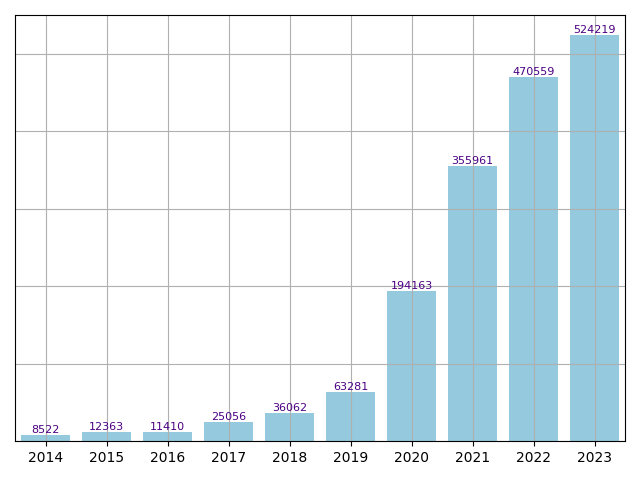
\includegraphics[width=\linewidth]{images/EV_amount.png}
	\end{center}
	\caption{Amount of new EVs on Road}
	\label{fig: ev_market}
	\captionsetup{font={footnotesize,bf,it}}
  	\caption*{Data: European Commission, \cite{Estat}} 
\end{figure}
Figure \ref{fig: ev_market} illustrates the number of newly purchased EVs in the market from 2014 to 2023. The most remarkable change, or rather 'boom', occurred in 2020. The most remarkable change, arguably a true boom, occurred in 2020. Coincidentally, 2020 was also the year of the COVID-19 outbreak. Germany has undergone astonishing changes over the past five years, but so far, we have only looked at EV-specific figures. To better understand the scale of this shift, let’s now consider the total number of newly registered vehicles overall.
\begin{figure}[H]
	\begin{center}
		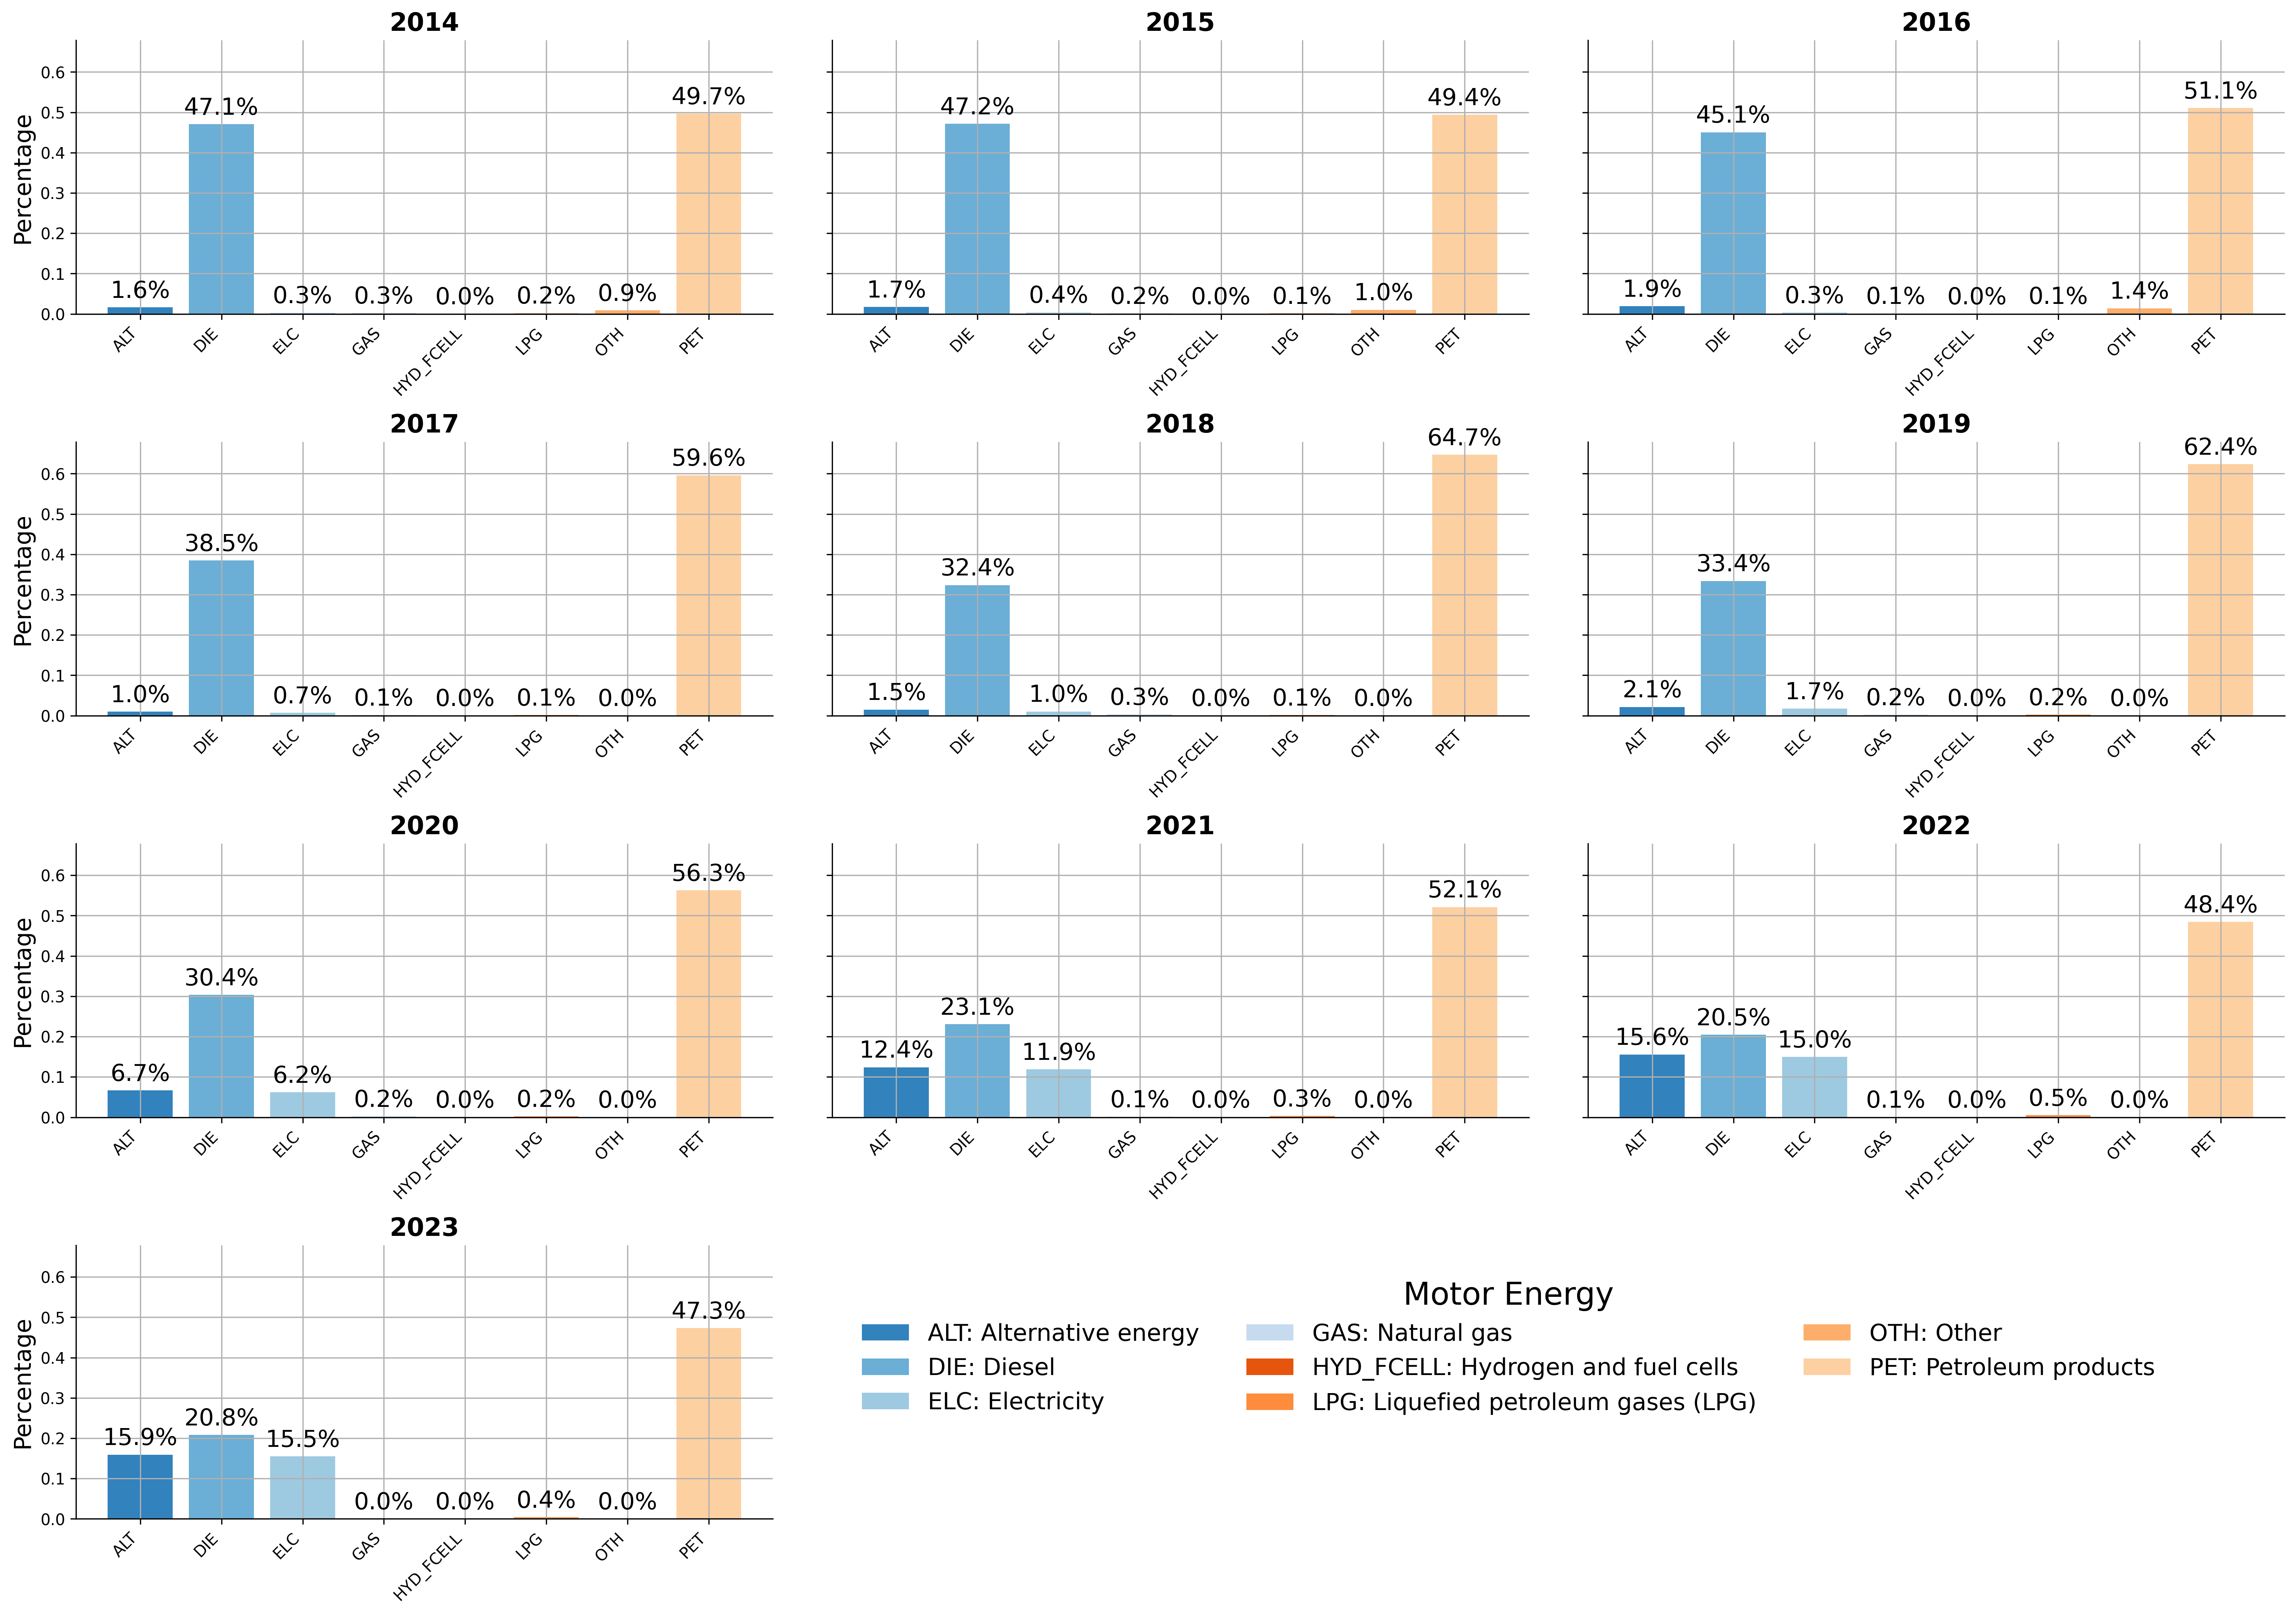
\includegraphics[width=\linewidth]{images/Veh_Mark.png}
		\caption{Percentage Distribution of Motor Energy Types in Vehicles Over Time}
		\label{fig: vehicles_market}
		\captionsetup{font={footnotesize,bf,it}}
  		\caption*{Data: European Commission, \cite{Estat}}
	\end{center}
\end{figure}
The development of electric mobility has been on a rise since 2016, s. Fig. \ref{fig: vehic_market}. It is important to note that the data excludes hybrid vehicles as their primary energy source remains fossil fuels. The most notable shift in the yearly share of newly registered electric vehicles occurred in 2020, with an increase of 5.7 percentage points. Another indicator of progress toward sustainable energy in the transport sector is the decline in both diesel and petrol vehicle registrations, accompanied by a steady rise in alternative powertrains. 

Another valuable dataset concerns the distribution of EVs between districts, s. Fig. \ref{fig: districts}. The disparity in EV ownership is evident when comparing East Germany—formerly the German Democratic Republic (GDR) under Soviet influence prior to reunification—with West Germany, which emerged as a prosperous free-market state after World War II. To this day, differences across various socio-economic categories between East and West Germany persist. A more detailed discussion on this topic can be found in \cite{BundestagOstWest}.
\begin{figure}[H]
	\begin{center}
		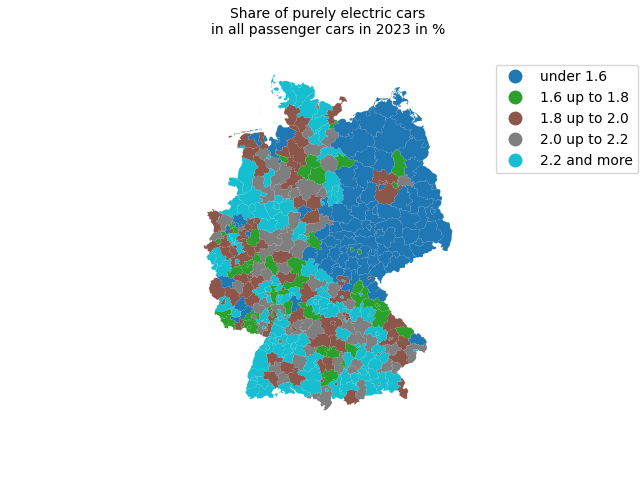
\includegraphics[width=\linewidth]{images/EV_percentage.png}
		\caption{Distribution of Electric Vehicles Across German Districts}
		\label{fig: districts}
		\captionsetup{font={footnotesize,bf,it}}
  		\caption*{Data: Deutschlandatlas, \cite{DeAtlasEVXLSX} \\
  				Map: BKG, \cite{BKG} } 
  	\end{center}
\end{figure}
The calculations below highlight the differences in EV ownership between densely populated urban areas and rural districts, s. Fig. \ref{fig: ev_percentage}. The values are based on the mean EV share within each category to ensure a representative comparison.
\begin{figure}[H]
	\begin{center}
		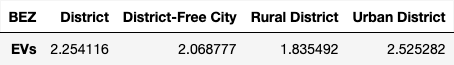
\includegraphics[width=\linewidth]{images/EVs_mean.png}
		\caption{Geographic Distribution of EV Ownership}
		\label{fig: ev_percentage}
		%\captionsetup{font={footnotesize,bf,it}}
  		%\caption*{Data: Deutschlandatlas, \cite{DeAtlasEVXLSX}}
	\end{center}
\end{figure}
Rural districts tend to have fewer electric vehicles compared to urban areas and cities, which could be attributed to limited charging infrastructure.
	